\section{Results and Conclusions}
\label{sec:make}

\subsection{Data}
  \label{sec:America}
  From the data collected of SW Lacertae the Magnitude over time is graphically displayed in the following depiction.
  \begin{figure}[H]
    \centering
    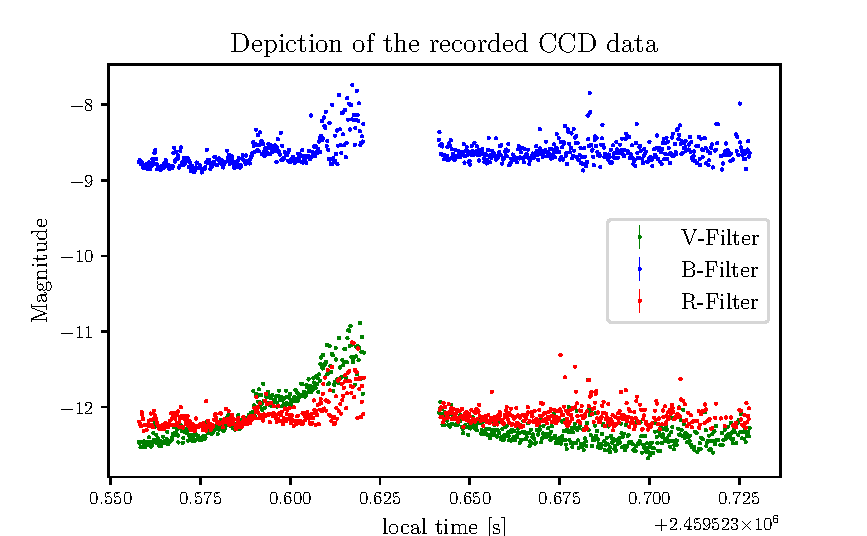
\includegraphics{Magnitude.pdf}
    \caption{Magnitude of SW Lacertae in B-, V-, and R-filters; 
    data was collected with a CCD array at 11 05 2021 (UT) at the $0.5$ meter Lutz telescope
    at Northern Arizona University}
  \end{figure}
  \noindent Additionally, data was collected of the two comparison stars. The gap in the data originates from when
  the meridian flip occurred. When an observed object crosses the meridian, the telescope has to be directed 
  to the other side of the sky (East and West). The slight diverge towards the meridian flip vanishes when taking the 
  difference of magnitudes from SW Lacertae and a comparison star. This is consistent with the 
  assumtion that it is a telescope or light disturbance artefact.\\
  \noindent The uncertainties in the following procedure were calculated with the package 
  uncertainties from python (Olivier et al.).
  
\subsection{Ensemble Photometry}
  \label{sec:great}
  The method of comparison stars was used in order to excluded errors as a result 
  from different exposures to external light sources. 
  Hence, the magnitude of the star was not utilized, but the difference between the star’s 
  magnitude and the magnitude of the comparison stars. For this study, the stars 
  (1) TYC 3215-1586-1 and (2) TYC 3215-1406-1 were chosen as comparison stars. 
  In the following image, their position in the sky in relation to SW Lacertae
  is depicted.
  \begin{figure}[H]
    \centering
    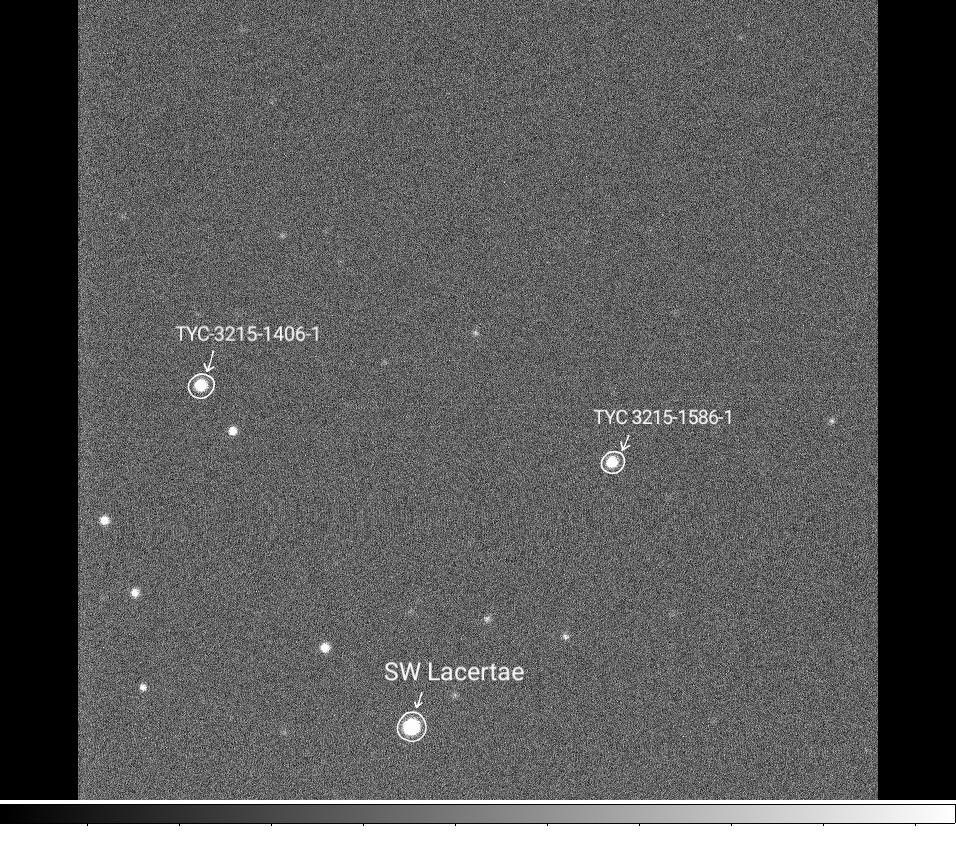
\includegraphics[width=200pt]{WestHA~2.jpg}
    \hspace{1em}
    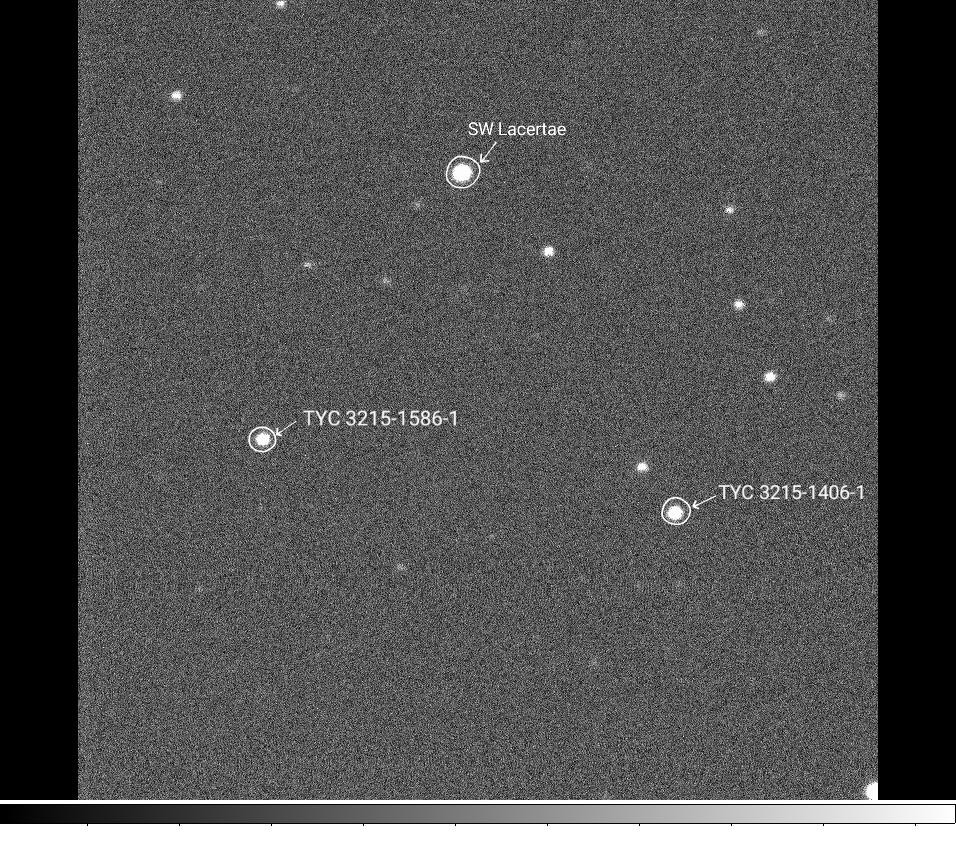
\includegraphics[width=200pt]{EastHA~2.jpg}
    \caption{Position of comparison stars in the sky; western sky on the left, eastern sky on the right}
    \label{fig:plot}
  \end{figure}
  \noindent The comparison to two stars was utilized to reduce the likelihood of 
  variation in the comparison star brightness and other intruding factors. The difference
  between the two comparison stars was calculated and didn't display a certain trend.
  Furthermore, the stationary brightness was looked up in the catalogue of the Centre de Données 
  astronomiques de Strasbourg (Wenger et al. 2000).
  This method was conducted for each filter seperately, because of the different 
  exposure times and colors of the stars.
  The resulting data for the V-filter is shown in the following plot.
  \begin{figure}[H]
    \centering
    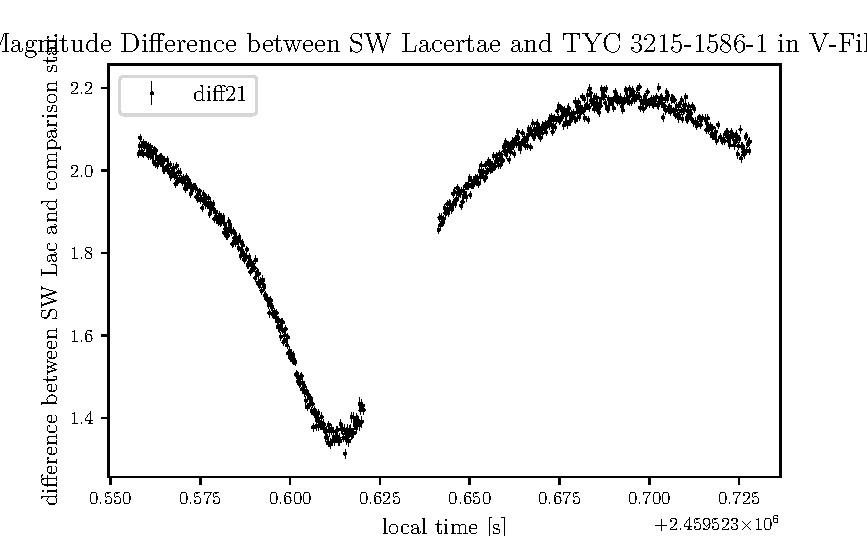
\includegraphics{V-Filter.pdf}
    \caption{Magnitude Difference between SW Lacertae and TYC 3215-1586-1 in V-Filter.}
    \label{fig:plot}
  \end{figure}

\subsection{Phase}
  \label{sec:again}
  In order to obtain the phase, in relation to a measured phase $49594.4684$ (, the first step is to calculate the epoch.
  \begin{equation*}
    E_{measurements} = HJD - 240000000
  \end{equation*}
  The data for an earlier Minimum was provided by the 
  instructions for this lab. 
  \begin{align*}
    E_{min} = 49594.4684\\
    period = 0.3207209
  \end{align*}
  The phase in comparison to the given data is retrieved through the formula:
  \begin{equation}
    phase = \dfrac{((E_{measurements}-E_{min})\ \% \ period)}{period}.
  \end{equation}
  This leads to the following results:
  \begin{figure}[H]
    \centering
    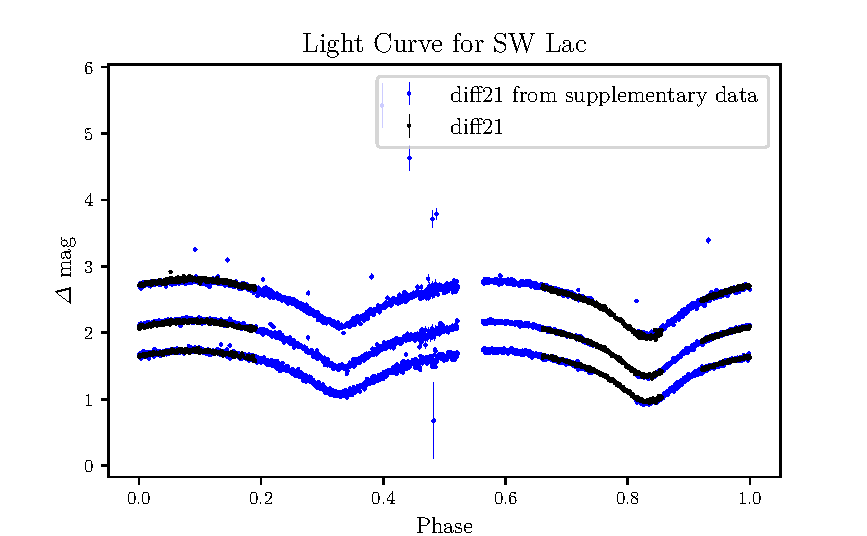
\includegraphics{gdPhase.pdf}
    \caption{Magnitude difference plotted against the Phase; contains data from another group. Their data is phase-shifted, so that it matches with our observations.}
    \label{fig:phase}
  \end{figure}
  \noindent As mentioned before, the smaller gap in our data is caused by the meridian flip. 
  Due to difficulties whith the telescope camera shutter, the observations had to be terminated
  before a whole period could be observed. Therefore, there is a bigger gap in the 
  data. For this reason, data gathered from another group was included to complete our graph. 
  They observed this binary star system at the same observatory the previous night. Since their
  observation, a phaseshift occured. In order to fill the gaps in our data,
  a phase of $+0.647$ was added. Due to the fact, that the supplementary data had other 
  comparison star and different exposure times, the light curves are also shifted in their
  magnitude. Therefore, the magnitude of the other groups data was also shifted
  by $-0.59$ for V-filter and $-0.56$ for B-filter.\\
 
\subsection{Conclusion}
  \label{sec:fuckoff}
  On account of difficulties, which occured while recording the data, a full period could not
  be observed. The conclusion is base primarily established on the data collected by the other team.
  The lightcurves of both observation nights coincide with each other and therefore, 
  it can be presumed, that the supplementary data will deliver results that match those of our 
  observations.\\
  \noindent It can be seen in figure \ref{fig:phase}, that there is an offset of the first minimum 
  and $phase = 0$ of $ 0.338$. That implies a period change of the system. As can be extracted from
  the other groups data, which had to be shifted by a phase of 
  $+0.674$, the period change is quite big. This developement should be 
  further researched, because it could lead to new knowlegde on mass transfer of contact binary
  star systems.\\
  \noindent As expected, the Minima are of different magnitudes. This is caused by the different brightness
  of the two stars. The discrepancy of the magnitudes of the Maxima has a different reason. The source 
  of this discrepancy lies in the McConnel effect. It is common for contact binary star systems 
  and is connected to cold star spots.

\subsection{Discussion}
  \label{sec:orange}
  \noindentThere were many factors that could have contributed to errors in the data we collected. This includes external light sources such as
  passing cars and street lights from the university. During observing, the camera shutter failed because of the short exposure times
  , and in turn streaks of light and dark patches were present in a majority of the data. This lead to an incomplete phase observation
  because our time was limited and we had to discard a lot of images. That is why it was necessary to use data from groups with the object SW Lac
  that we're able to collect a complete phase. Many uncertainties were also considered but not completely mitigated such as the auto guider, atmospheric changes, dust particles, and our bias images. We analyzed our observations, and although limited, the data was consistent with the additional data provided by Gordon Hageman and Cameron Piotti.
  
\section{Acknowledgements}
(( not sure what the label should be ))

\noindent We would like to acknowledge the Atmospheric Research Observatory and the operators who helped us collect our data. We would like to thank Gordon Hageman and Cameron Piotti for generously sharing their data so we could complete our phase curve. We would like to thank Edwin Anderson for allowing us this opportunity to carry out this research. 
